\chapter{Methods}
\label{sec:methods}

\section{\NoCaseChange{\acl{RXTE}}}
While a number of X-ray missions have been conducted over the years, \ac{RXTE} remains a unique mission due to its extraordinary timing resolution \citep{bradt1993x}. Operating for more than 16 years from 1995 to 2012, \ac{RXTE} built up a significant archive of transient X-ray sources, providing a large repository of \ac{LMXB} observations \citep{heasarc}. Using the \ac{HEASARC} online services, provided by the NASA/Goddard Space Flight Center, data can freely be downloaded for the full length of the mission. With a wide range of data types available, the variety in data products originates in the different instruments carried on board \ac{RXTE}.\\

\ac{RXTE} carried out observations with three observational instruments -- the \ac{ASM}, the \ac{HEXTE} and the \ac{PCA} \citep{bradt1993x}. The \ac{ASM} was designed to survey a large fraction of the sky every 1.5 hours, allowing the intensity and spectrum of more than 75 objects to be monitored. Upon rapid changes in either property, the \ac{HEXTE} and the \ac{PCA} could be pointed towards the target typically within a few hours. The energy ranges of the \ac{HEXTE} and the \ac{PCA} were designed to be complimentary, with the \ac{HEXTE} observing from 15-200 keV, and the \ac{PCA} from 2-60 keV \citep{jahoda1996orbit}. Both instruments had a $1^\circ$ field of view, and a minimum timing resolution of $8\mu$s for the \ac{HEXTE} and $1\mu$s for the \ac{PCA} \citep{rothschild1998flight, zhang1993laboratory}. \\

Only observations conducted with the \ac{PCA} are used throughout this project, providing an extensive source of data. Comprised of five \acp{PCU}, the \ac{PCA} allowed energies to be determined to an energy resolution of less than 18\% at 6~keV \citep{pcainfo}. Each \ac{PCU} was filled with a mixture of Xenon and Methane gas, allowing charged particles to ionise the gas, resulting in an electrical pulse proportional to the energy carried by the incident particle \citep{zhang1993laboratory}. An additional layer on top of each \ac{PCU} contained propane gas in order to reduce the effect of background events. A gradual loss of propane occurred at the start of the mission, leaking through to the Xenon layers \citep{jahoda1996orbit}. Combined with other effects, this resulted a gradual change in gain for which gain epochs have to be defined to correct for these changes \citep{rxteenergychannel}. The loss of the PCU$0$ propane layer in 2000 required the adoption of an additional calibration epoch. An internal radioactive source allowed for continuous energy calibration \citep{zhang1993laboratory}.\\

With each active \ac{PCU} providing data, information was sent to six \acp{EA} incorporated in the \ac{EDS} \citep{jahoda1996orbit}. This phase allows for data processing and compression before telemetry. Two of the \acp{EA} were programmed to run in standard configurations, with the others able to run in one of the seven different modes \citep{rxtepcaissues}. The sheer number of options, and parameters, needed to extract this data from the different modes requires a large set of extraction tools. With the previous paragraphs giving a brief overview of the hardware behind the observations, additional technical details on the \ac{PCA} can be found in \citet{zhang1993laboratory}. Shifting to the data extraction and analysis side of data reduction requires specialised software, and is explained in the following section.\\

\section{Data Reduction}
\label{sec:data_reduction}
In order to conduct a systematic population study, a robust pipeline is needed to run through many scores of observations. While a number of tools are available to help in extracting data, these tools do not lend well to upscaling, often requiring a large number of input parameters for every data mode. To this end, the \chromos software pipeline was developed. The technical side of \chromos is described in appendix~\ref{ch:chromos}, in the form of a manual, with information on the underlying methods presented in this section. \ \\

The \ac{HEASARC} online services provides several interfaces for searching and retrieving \ac{RXTE} data \citep{rxtearchive}. Using the web-based graphical user interface, a list of ObsIDs can be obtained for each target. ObsIds are used to classify observations, and are an identification code which changes when a new target is acquired, or when the \ac{EA}-modes change. ObsIDs follow the format of 'NNNNN-TT-VV-SSX', with NNNNN a five-digit proposal number, TT a two-digit target number, VV a two-digit viewing number, SS a two-digit number to identify different pointings and X a character to denote slewing, configuration changes etc \citep{rxtearchive}. An \sw{ftp}-server allows for downloads to be conducted via the command line. Extracting this data requires some knowledge of the available data modes per observation. Two \acp{EA} modes should be permanently available, \sw{standard1} with no energy information but a 0.125s timing resolution and \sw{standard2} data with 129 spectral channels and a 16s time resolution \citep{rxtestdproducts}. A whole range of other data modes can also be present depending on the observation. These modes fall into two categories - science array (also known as binned-mode data) and science event format. Both formats require different tools and input to extract the data. Science array format includes data modes such as \sw{binned} and \sw{standard2}, and science event format, data modes such as \sw{good\-xenon} and \sw{event} mode. Each data mode can provide diverging timing resolutions depending on the binning method, but files must have a timing resolution higher than $\sfrac{1}{128}\ $s for our subsequent analysis, with the exception of files for spectral analysis and background creation. \\

To ensure data remains a reliable reflection of the actual target emission, it must be filtered using \acp{GTI} \citep{rxtecookbookevent}. Following the \ac{RXTE} cookbooks for science array and science event mode data, the ftool \sw{maketime} is used to set filter criteria \citep{maketime,rxtecookbookbinned,rxtecookbookevent}. To ensure the earth brightness does not contaminate observations, the pointing elevation is set to be above $10^\circ$. Additionally, the pointing offset is set to be less than $0.02^\circ$ and the number of active \acp{PCU} set to be greater than one. For all objects save for black holes and Sco~X-1, up to 10min since the \ac{SAA} is removed \marginpar{The \ac{SAA} refers to an area in which the Earth's magnetic field is reduced in strength, causing an increase in high energy particle count rates \ \ \ \ \citep{saa}.} and an electron count larger than 0.1 is removed to prevent electron contamination. The former sources show sufficiently high count rates to neglect this last criterion, and with current backgrounds able to account for the \ac{SAA} passage, the filtering on time since \ac{SAA} is not required. Using information from standard filter files, the times at which a change in number of \acp{PCU} occurs are noted, allowing for 32s around these transitions to be filtered during extraction. This prevents any surge, or change in electrical current, from contaminating the count rate. \\

Background files are created from \sw{standard2} files together with standard filter files using the ftool \sw{pcabackest} \citep{pcabackest}. This estimated background spectrum also requires a provided model file. With sources showing a net count rate larger than 40~ct/s/PCU, the 'bright' background model can be used for all sources \citep{pcadigest}. Having created background files, the sole step left before extracting the main data files, is determining the correct energy channel ranges. This final part is potentially the most complicated part of \chromos, requiring a number of steps. On the basis of the observation date, an initial channel range can be selected using the energy-channel conversion table \citep{rxteenergychannel}. If files are in \sw{event} or \sw{binned} mode, then the header of these files will show the channel binning, which can vary from observation to observation. The final channels can be selected using this information, in which channel bins closest to the energy range 2-13~keV are selected while ensuring the lowest energy channels are omitted \citep[see][]{gleissner2004long}.\\

Extracting data requires two ftools: \sw{saextrct} for \sw{event} and \sw{goodxenon} files and \sw{seextrct} for \sw{standard2} and \sw{binned} files \citep{saextrct,seextrct}. The input parameters can be determined using the files and information generated in the previous steps, with exception of the timing resolution. This is set to $\sfrac{1}{128}\ $s for all files save for \sw{standard2} files, which are extracted with their intrinsic resolution of 16s. A background file is extracted for each subsequent data file to ensure the same filter criteria are applied. \sw{standard2} files are extracted for PCU2 only, the sole PCU with an intact propane layer of the course of the mission, and the most stable one. While the low timing resolution of \sw{standard2} files prevents any high precision timing analysis from taking place, this data is well-suited to spectral analysis. \sw{standard2} files are therefore extracted as both spectra and light curves, rather than just as light curves as all other data modes are.\\

\section{Timing Analysis}
\label{sec:timing_analysis}
Light curves must be background corrected, which necessitates the rebinning of background light curves to match the resolution of the original light curve files. This is done on basis of interpolation between each consecutive background data point. Subtracting these values from the light curve count rates produces a light curve suitable for further analysis. To prevent the flares from affecting the general variability trend throughout a single observation, X-ray bursts are identified and removed for all neutron star systems. Tests showed that two consecutive count rates above a \acf{RMS} per observation of 7$\sigma$ provided a strong indication for an X-ray burst. Numerous methods for automatically identifying the start and end of the bursts were tested, but in the end a choice was made to cut fixed time bins on other side. Approximately 3s was cut before each detection, and 625s afterwards. Further discussion on this method can be found in section~\ref{sec:dis_bursts}.\\

In order to conduct timing analysis, a switch must be made to the frequency domain. Unless specified elsewhere, all following information is based on work presented in \citet{uttley2014x}. While a variety of techniques are available to conduct time-series analysis \citep[e.g.][]{maccarone2000time,legg2012direct}, discrete Fourier transforms are the most prevalent. These transforms can be calculated with
\begin{align} 
X_n = \sum^{N-1}_{k=0}x_k\ e^{\sfrac{2\pi ink}{N}}
\end{align}
with $X_n$ the discrete Fourier transform, $N$ the number of time bins and $x$ the $k^\textrm{th}$ value of the light curve. $X_n$ is calculated in steps of $f_n=\sfrac{n}{N\Delta t}$ with $\Delta t$ the width of a time bin and with $n=0,1,2\ldots \sfrac{N}{2}$. The maximum frequency is thus 64~Hz due to the $\sfrac{1}{128}\ $s time resolution of the extracted light curves. In order to obtain a power spectrum, the discrete Fourier transform is multiplied with its complex conjugate
\begin{align}
|X_n|^2 = X_n X_n^*
\end{align}
The resulting power spectrum is subsequently normalised with
\begin{align}
P_n = \frac{2\Delta t}{\langle x \rangle ^2 N}|X_n|^2
\end{align}
in which $\langle x \rangle$ is the mean flux of the light curve. This leads to units in terms of fractional variance per Hz \citep{belloni1990variability}. With the exception of perhaps an \ac{AMSP}, few sources show fully periodic signals over all observations, but will usually show shifting power spectral components. A decision must therefore be made on the total time over which to Fourier transform. With power spectra errors dependent on the number of power spectra over which is averaged, a trade-off is established. Reducing the noise on the final power spectrum requires averaging over many segments, but in the process reduces the sensitivity to varying power spectral components. Following the procedure given in \citet{heil2015power}, a choice is made to take discrete Fourier transforms of each $m^{th}$ segment of 512s in an observation, and average these power spectra:
\begin{align}
\overline{P}_n = \frac{1}{M} \sum_{m=1}^M P_{n,m}
\end{align}
in which $M$ is the total number of segments in an observation. This number is limited not just by the total length of the light curve, but also by gaps due to PCU changes, X-ray bursts etc. The decision to bin across each observation is expanded on in section~\ref{sec:binning}, where alternative binning methods are also discussed. \\
\clearpage
With power spectra flattening towards higher frequencies, a correction can be applied by calculating the white noise present in the power spectrum with
\begin{align} 
P_\textrm{noise} = 2\frac{\langle x \rangle + \langle b \rangle}{\langle x \rangle ^2} \label{eq:noise}
\end{align}
in which $\langle x \rangle$ is the mean count rate and $\langle b \rangle$ is the mean background count rate in $\overline{P}_n$. The resulting noise value can be subtracted from the power spectrum. The associated errors on the noise corrected power spectrum are then calculated by dividing each power by $\sqrt{M}\hspace{2pt}$. As the powers are $\chi^2_2$-distributed, errors on the power spectrum can be approximated as Gaussian provided a large number of samples are binned.\\

Power spectral evolution can be parametrised using power colours, as described in section~\ref{sec:commontechniques}. These can be calculated using the power spectra obtained for each observation. First, the integrated power, or variance $V$, can be calculated using
\begin{align} 
V = \Delta \nu \sum_{i=\nu_\textrm{low}}^{\nu_\textrm{high}} \overline{P}_i
\end{align}
with $\Delta \nu$ the Nyquist frequency and $\overline{P}_i$ the power in frequency $i$, running between the four equally spaced frequency bands of 0.0039-0.031~Hz, 0.031-0.25~Hz, 0.25-2.0~Hz and 2.0-16.0~Hz \citep{heil2015power}. This results in a variance value $V$ for each consecutive frequency band, respectively referred to as $V_A$, $V_B$, $V_C$ and $V_D$. Defining two power colours as
\begin{align}
	PC1 = \frac{V_C}{V_A} \hspace{20pt} \textrm{and} \hspace{20pt} PC2 = \frac{V_B}{V_D} 
\end{align}
allows an observation to be placed in a \ac{PCC}~diagram, with $PC1$ on the horizontal axis and $PC2$ on the vertical axis. The associated error values can be calculated from the errors on the variance, determined with
\begin{align}
Err^2(V) = \frac{(\Delta \nu)^2}{M} \sum_{i=\nu_\textrm{low}}^{\nu_\textrm{high}} \overline{ P^2 }_i
\end{align}
as given by \citet{heil2012ubiquity}. Note that the summation is over the average squared power, rather than over the squared average power. Power colour errors can subsequently be calculated with simple error propagation
\begin{align}
Err(PC1) = PC1 \sqrt{\left(\frac{Err(V_C)}{V_C}\right) ^2 + \left(\frac{Err(V_A)}{V_A}\right) ^2}
\end{align}
and $Err(PC2)$ in analogous fashion.

\section{Spectral Analysis}
Spectral analysis is conducted with \sw{standard2} files, due to both their energy resolution, and their relative ease of use. The ftool \sw{pcarsp} is run for all files prior to any analysis, allowing response files to be created from energy spectra and filter files \citep{pcarsp}. These response files can be used by the X-ray spectral-fitting program \sw{xspec} \citep{arnaud1996astronomical} to ensure an accurate representation of count rates in each energy bin after subtracting background values. Energies outside the range 2-13~keV are ignored, before unfolding the energy spectrum around a flat powerlaw. In doing so, the energy spectrum is effectively being divided by the effective area of the instrument response, providing energy spectra independent of long term changes in instrument response \citep{heil2015inclination}. The energy spectral hardness is calculated for a variety of energy bands, by integrating the count rate over energy and dividing the resulting flux of the higher energy band by that of the lower energy band. These fluxes are additionally summed, to obtain the relative total intensity.\\

%TODO Error calculation for integrating over energies? Does this paragraph need any formula's?

\section{Targets}
In order to compare the variability properties of both black hole and neutron star \acp{LMXB}, a selection of objects is required. An overview of the chosen objects can be found in Tab.~\ref{tab:objects} and includes information on various system parameters. The choice of objects was based primarily on the number of \ac{RXTE} observations available, but also on the system type. These were chosen to ensure a good spread across both atoll and Z sources, as well as various inclinations, accretion states etc. Sources have been divided by compact object, with neutron stars above the centre line, and black holes below. Most columns should be self-explanatory, however \spacedlowsmallcaps{\#Good} may require additional explanation. This refers to the number of ObsIDs which have power colour ratios with a fractional variance constrained at a 3$\sigma$-level in each frequency band. Further discussion on these values can be found in section~\ref{sec:selection_criteria}, in which various selection effects are examined. The object names used in this table and throughout this thesis were selected to reflect the most common name in use. Alternate source names can however be found in Tab.~\ref{tab:aka}, presenting source designations from the \sw{4U}, \sw{GX}, \sw{IGR}, \sw{INTEGRAL1}, \sw{SWIFT}, \sw{X} and \sw{XTE} catalogues \citep{SIMBAD}. The choice of black holes systems was made on basis on of \ac{PCC}~diagram coverage as presented in \citet{heil2015power}, providing a representative sample of possible black hole power colour tracks. \\


\section{Robustness of \chromos}
Initial tests of the pipeline were conducted by comparing power colours of Aql~X-1 with prior results presented in \citet{heil2015power}. Both the results can be seen in Fig.~\ref{fig:aqlx1}, with left showing power colours from \citet{heil2015power} and right showing results obtained with \chromos. Similar tracks are found for Aql~X-1 with both methods, save for the top left corner of the \ac{PCC}~diagram where observations are primarily in the soft state. A close inspection revealed differences in noise correction, where \citep{heil2015power} used spectral fitting to obtain the white noise, in contrast to the approach taken in this work. Additional binning effects also played a role, and are discussed further in section~\ref{sec:binning}. The power colours track of black holes obtained with \chromos showed only minor differences in comparison to those obtained in \citet{heil2015power}. Further tests were also conducted on parameters related to energy spectra, revealing similar hardness and intensity values in past spectral studies. Suggestions on scientific improvements to \chromos are given in the discussion, section~\ref{ch:discussion}, with coding recommendations in appendix~\ref{ch:chromos}.

\begin{figure}%
\myfloatalign%
\makebox[\textwidth][r]{%
\subfloat{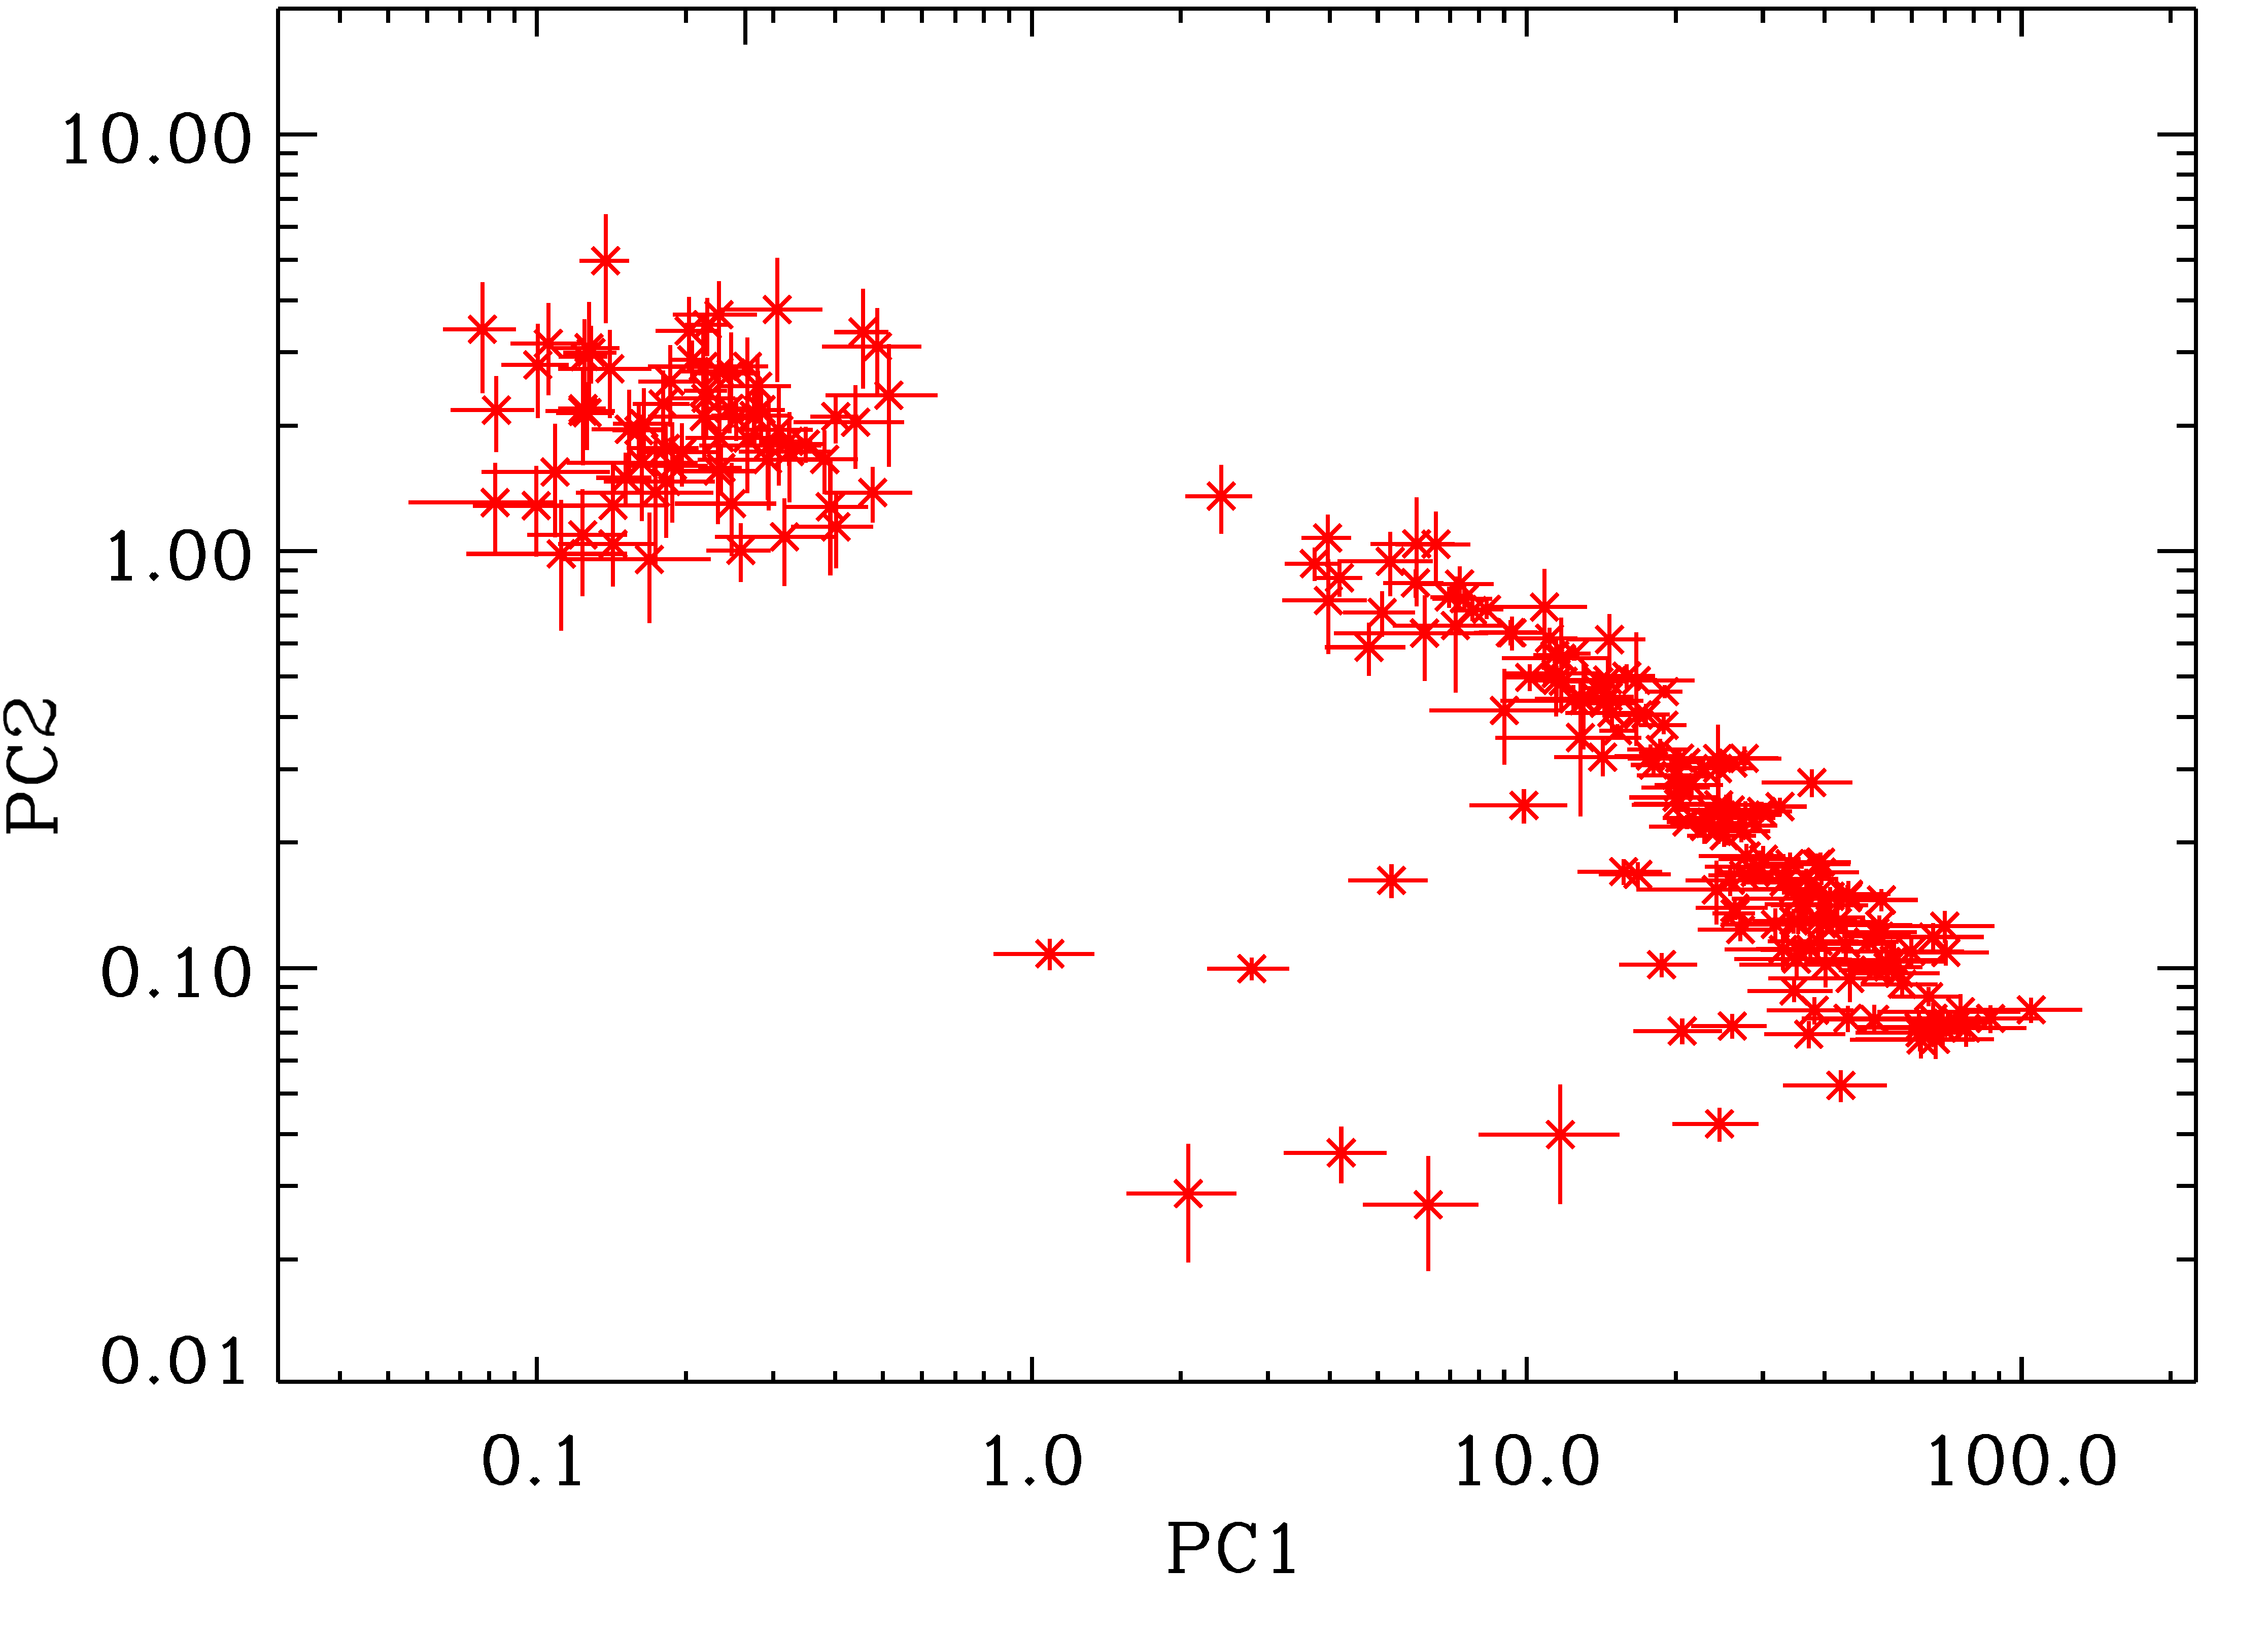
\includegraphics[width=.42\largefigure,valign=t]{pc/aquila_lucy.png}}%
\quad%
\subfloat{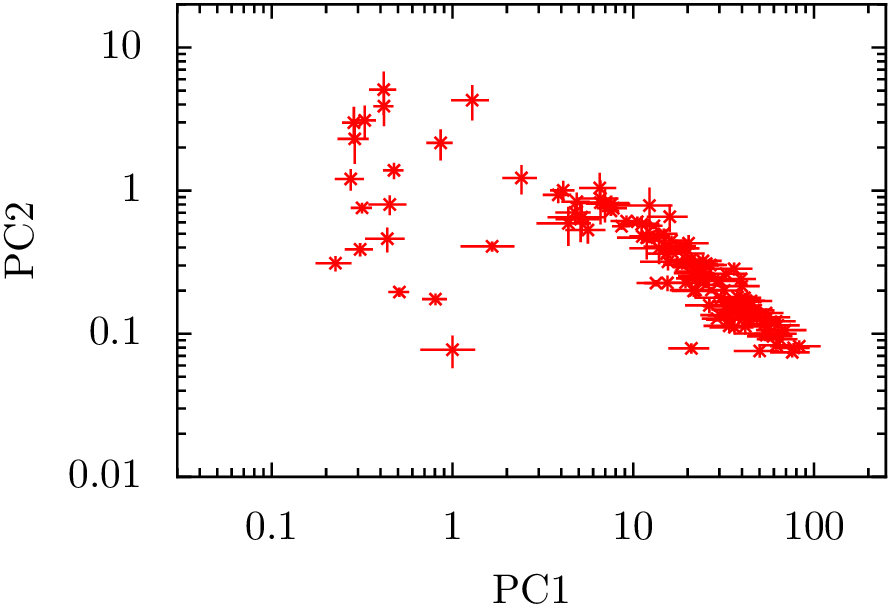
\includegraphics[width=.45\largefigure,valign=t]{pc/individual/aquila_X1}}%
}%
\caption[Comparison of Aql~X-1 \acs{PCC}~diagrams]{\spacedlowsmallcaps{left} Power colour ratios obtained for Aql~X-1 by \citet{heil2015power}. To ensure clarity, the original figure has been adapted by removing power colours from black hole systems. \spacedlowsmallcaps{right} Power colour ratios obtained with \chromos for Aql~X-1. Only power colours with a fractional variance constrained at a $3\sigma$ level in each frequency band have been included.}\label{fig:aqlx1}
\end{figure}

\newcolumntype{L}[1]{>{\raggedright\let\newline\\\arraybackslash\hspace{0pt}}m{#1}}
\newcolumntype{C}[1]{>{\centering\let\newline\\\arraybackslash\hspace{0pt}}m{#1}}
\newcolumntype{R}[1]{>{\raggedleft\let\newline\\\arraybackslash\hspace{0pt}}m{#1}}

%\setlength{LTcapwidth}{10.in}
\begin{landscape}
\begin{longtable}{@{\extracolsep{\fill}}>{\centering\arraybackslash}p{4cm}ccccccc@{}}
\caption[Object properties]{Overview of \acp{LMXB} showing system properties and observation details, sorted by compact object type, and then by name. Alternative source names can be found in appendix~\ref{ch:sources}, in table~\ref{tab:aka}. Systems are divided into atolls (A), Z sources (Z), accreting pulsars (AP), accreting millisecond pulsars (AMP), and objects showing characteristics of both atoll and Z sources (AZ). A further division is made between persistent accretion-powered pulsars with burst oscillations (P), intermittent ones (I) and burst oscillation sources without detectable accretion-powered pulsations (B) \citep[see][for a review]{watts2012thermonuclear}. Intermittent sources have been assigned to the pulsar or burster group on basis of their timing properties \citep{marieke}. Spin frequencies have been given where possible, as are inclination angles. \spacedlowsmallcaps{\#Good} gives the total number of observations with a significant detected variance at a 3$\sigma$-level in all four power colour frequency bands. The total number of available ObsIDs in the \ac{RXTE} archive are also given per source. References are denoted with numbers, and are given at the bottom of this table.}\label{tab:objects}\\
\multicolumn{8}{l}{} \\[-7pt]
\toprule
\tableheadline{Source}&\tableheadline{Type}&\tableheadline{Burster/Pulsar}&\tableheadline{Spin Freq. (Hz)}&\tableheadline{Inclination ($^\circ$)}&\tableheadline{\#Good}&\tableheadline{\#ObsID}&\tableheadline{References}\\
\midrule
\endfirsthead
\toprule
\tableheadline{Source}&\tableheadline{Type}&\tableheadline{Burster/Pulsar}&\tableheadline{Spin Freq. (Hz)}&\tableheadline{Inclination ($^\circ$)}&\tableheadline{\#Good}&\tableheadline{\#ObsID}&\tableheadline{References}\\
\midrule
\endhead
4U 0614+09&A&B&414.7&86&85&502&1,2,2,3\\
4U 1636-53&A&B&581.9&64&45&1556&4,5,2,6\\
4U 1702-43&A&B&329&&28&210&7,5,5\\
4U 1705-44&A&&&51&55&516&8,9\\
4U 1728-34&A&B&363&50&55&405&7,5,5,10\\
Aql X-1&A&I/B&550.3&72–79&145&596&4,5,2,11\\
Cir X-1&AZ&&&90&52&811&12,13\\
Cyg X-2&Z&&&62.5&62&567&8,14\\
EXO 0748-676&A&B&552.5&75&93&746&15,5,16,17\\
GX 17+2&Z&&&&4&206&8\\
GX 340+0&Z&&&&5&97&8\\
GX 349+2&Z&&&&3&142&8\\
GX 5-1&Z&&&&5&167&8\\
HETE J1900.1-2455&AMP&I/P&337.3&30&129&361&18,5,19,20\\
IGR J00291+5934&AMP&&599&&45&479&21,22\\
IGR J17480-2446&AP&P&11&&42&159&23,5,23\\
IGR J17498-2921&AMP&P&401&&3&129&24,5,24\\
KS 1731-260&A&B&524&&21&82&7,5,5\\
SAX J1808.4-3658&AMP&P&401&55&25&1337&25,5,25,26\\
SWIFT J1756.9-2508&AMP&B&182&&19&50&27\\
Sco X-1&Z&&&30&48&598&8,28\\
Sgr X-1&A&&&&12&109&8\\
Sgr X-2&Z&&&&35&88&12\\
V4634 Sgr&A&&&&119&1008&29\\
XB 1254-690&A&&&&10&94&30\\
XTE J0929-314&AMP&B&185&&7&46&31,31,22\\
XTE J1701-462&AZ&&&60&94&872&12,28\\
XTE J1751-305&AMP&B&435&&21&274&32\\
XTE J1807-294&AMP&P&190&&4&112&33,2,22\\
XTE J1814-338&AMP&P&314&&17&93&34,5,22\\
\midrule
\\[-20pt]
GX 339-4&BH&&&&391&1401&35\\
H1743-322&BH&&&&123&558&36\\
XTE J1550-564&BH&&&&141&423&37\\
\bottomrule
\\[-7pt]
\multicolumn{8}{L{23cm}}{
\spacedlowsmallcaps{1}~\citet{mendez1997kilohertz} \spacedlowsmallcaps{2}~\citet{marieke} \spacedlowsmallcaps{3}~\citet{schulz2010dynamical} \spacedlowsmallcaps{4}~\citet{liu2001catalogue} \spacedlowsmallcaps{5}~\citet{watts2012thermonuclear} \spacedlowsmallcaps{6}~\citet{pandel2008relativistic} \spacedlowsmallcaps{7}~\citet{galloway2008thermonuclear} \spacedlowsmallcaps{8}~\citet{hasinger1989two} \spacedlowsmallcaps{9}~\citet{di2009relativistically} \spacedlowsmallcaps{10}~\citet{shaposhnikov2002bursting} \spacedlowsmallcaps{11}~\citet{galloway2016intermittent} \spacedlowsmallcaps{12}~\citet{fridriksson2015common} \spacedlowsmallcaps{13}~\citet{iaria2008chandra} \spacedlowsmallcaps{14}~\citet{orosz1999optical} \spacedlowsmallcaps{15}~\citet{homan2015geometric} \spacedlowsmallcaps{16}~\citet{galloway2010discovery} \spacedlowsmallcaps{17}~\citet{parmar1986discovery} \spacedlowsmallcaps{18}~\citet{watts2009discovery} \spacedlowsmallcaps{19}~\citet{morgan2005hete} \spacedlowsmallcaps{20}~\citet{papitto2013accretion} \spacedlowsmallcaps{21}~\citet{galloway2005discovery} \spacedlowsmallcaps{22}~\citet{gladstone2007analysing} \spacedlowsmallcaps{23}~\citet{papitto2011spin} \spacedlowsmallcaps{24}~\citet{papitto2011discovery} \spacedlowsmallcaps{25}~\citet{wijnands1998millisecond} \spacedlowsmallcaps{26}~\citet{cackett2009broad} \spacedlowsmallcaps{27}~\citet{krimm2007discovery} \spacedlowsmallcaps{28}~\citet{crampton1976spectroscopic} \spacedlowsmallcaps{29}~\citet{van2005relations} \spacedlowsmallcaps{30}~\citet{bhattacharyya2007timing} \spacedlowsmallcaps{31}~\citet{galloway2002discovery} \spacedlowsmallcaps{32}~\citet{markwardt2002discovery} \spacedlowsmallcaps{33}~\citet{markwardt2003discovery} \spacedlowsmallcaps{34}~\citet{markwardt2003xte} \spacedlowsmallcaps{35}~\citet{wijnands1999broadband} \spacedlowsmallcaps{36}~\citet{homan2005high} \spacedlowsmallcaps{37}~\citet{homan2001correlated}
} \\
\end{longtable}
\end{landscape}
% 
% \begin{table}
%     \myfloatalign
%   \begin{tabularx}{\textwidth}{Xccc} \toprule
%     \tableheadline{Source}	& \tableheadline{Inclination}	& \tableheadline{Type (A/Z[Sco/Cyg])} & \tableheadline{Dipper} \\
%     \midrule
%     \TODO & \TODO & \TODO & \TODO\\
%     \midrule
%     \TODO & \TODO & \TODO & \TODO\\%\citeauthor{knuth:1976} \\
%     \bottomrule
%   \end{tabularx}
%   \caption[\TODO]{\TODO}\label{tab:objects}
% \end{table}